%% 
%% LaTeX Boilerplate (http://github.com/gbluma/latex-boilerplate/)
%% 

\documentclass[12pt,fleqn,leqno,letterpaper]{article}
\usepackage{graphicx}
\usepackage{amsmath}

\usepackage[scale=0.8, bmargin=2cm, tmargin=2cm, lmargin=3cm, rmargin=3cm]{geometry}
\title{Ca\_bot Inverse Kinematics}
\author{Antoine Pirrone\\
  \small{\texttt{antoine.pirrone@gmail.Com}}
}
\date{\today}

\begin{document}

\maketitle

\begin{figure}[h]  
  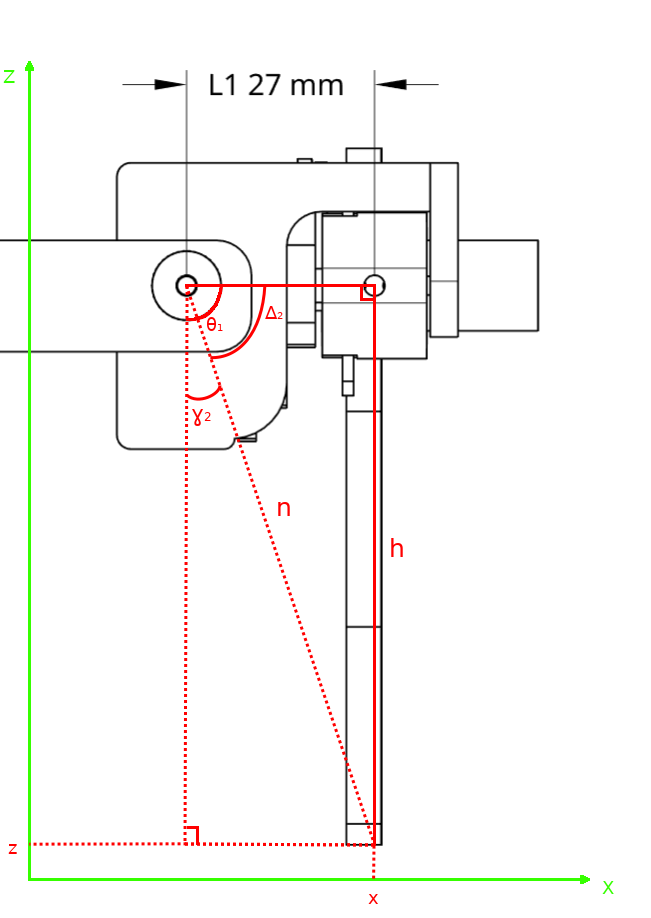
\includegraphics[scale=0.35]{assets/front_annotated.png}
  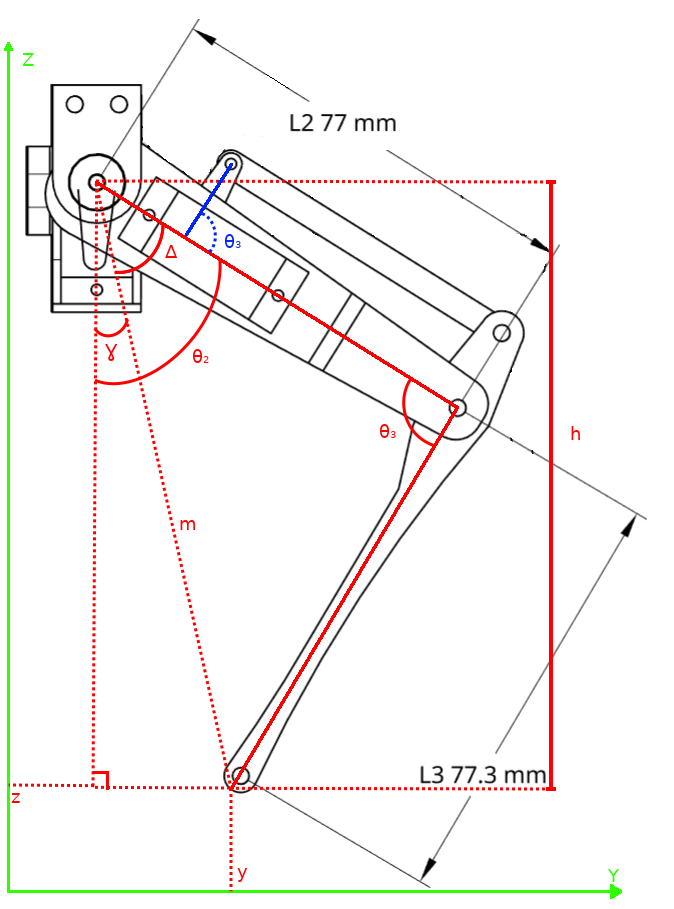
\includegraphics[scale=0.35]{assets/right_annotated.png}
  \caption{We use trigonometry to compute the inverse kinematics of the leg}
  \label{schematics}
\end{figure}

We want to find the values of the angles $\theta_{1}$, $\theta_{2}$ and $\theta_{3}$ given the $x$, $y$ and $z$ position of the end of the leg (see Figure \ref{schematics}).\\

\noindent For $\theta_{1}$, we first need to compute the angles $\gamma_{2}$ and $\Delta_{2}$. Using the Pythagorean theorem, we have : \\

\noindent$ n = \sqrt{z^2 + x^2}$ \\
$h = \sqrt{n^2 - L1^2}$\\

\noindent Which allow us to compute $\gamma_{2}$ :\\

\noindent $\gamma_{2} = \arcsin(\frac{x}{n})$\\

\noindent And $\Delta_{2}$ using Al-Kashi's theorem : \\

\noindent $\Delta_{2} = \arccos(\frac{-h^2 + n^2 + L1^2}{2 \cdot n \cdot L1})$\\

\noindent Then, \\

\noindent $\boxed{\theta_{1} = \gamma_{2} + \Delta_{2}}$\\

\noindent Same process for $\theta_{2}$, this time we need to compute $\gamma$ and $\Delta$. Using the Pythagorean theorem, we have : \\

\noindent $m = \sqrt{y^2 + h^2}$\\

\noindent Thus,\\

\noindent $\gamma = \arcsin(\frac{y}{m})$\\

\noindent And using Al-Kashi's theorem again : \\

\noindent $\Delta = \arccos(\frac{-L3^2 + m^2 + L2^2}{2 \cdot m \cdot L2})$\\

\noindent Then, \\

\noindent $\boxed{\theta_{2} = \gamma + \Delta}$\\

\noindent Eventually, we find $\theta_{3}$ using Al-Kashi's theorem again : \\

\noindent $\boxed{\theta_{3} = \arccos(\frac{-m^2 + L2^2 + L3^2}{2 \cdot L2 \cdot L3})}$\\

\noindent \textbf{Note} : The blue $\theta_{3}$ on Figure \ref{schematics} is the actual angle being actuated, but as we have a parallel mechanism here, it is actually the same value as the red one.

\end{document}
